\chapter{Usability}

\section{Aspects of Usability (OK tittlel???)}
Usability says something about how easy it is to use, learn and understand a human-made system. Examples of systems can be a machines, software applications, websites, tools, or anything else that involves human interaction with an object. Usability is often used in association with technology development, in terms of making digital systems understandable and intuitive for the users through user-friendly interfaces. Usability has played a huge part in the evolvement of bringing digital systems into people's homes and everyday life. The first computers and digital systems that were developed consisted of complex and not understandable applications that only professionals with special knowledge could use. There was little focus on simple and accessible systems, and complex interfaces were actually appreciated and gave the system credibility. First, when computers and digital systems were developed with the intention of being used by the normal user, developers had to think about usability. The developers had to put the user in the center of the computer system, and not only focus on functionality and system features \cite{mmi}.

We have experienced a great shift in technology from the first computer was invented and until today. Technology has been more mobile due to laptops, smart phones and other portable devices, and it is also used more often because of instant messaging, e-business and social networks \cite{mmi}. Users are no longer just "computer professionals", but normal people in all age groups, with different skills and interests, that are both experienced and inexperienced with technology. This has been possible because of designers and researchers with focus on human needs. The term human-computer interaction was created, which is about including psychology in developing human-centric design. This is not an easy task, and it includes people from  many different sciences. Ben Shneiderman lists "psychologist, instructional and graphic designers, technical writers, experts in human factors or ergonomics, information architects, and adventuresome anthropologists and sociologist" as people to be included in the process of saying something about usability and human-computer interaction \cite{mmi}.  

Usability is a wide and quite abstract term, and it is not easy to understand, to measure, or to practise right. ISO 9241-11 states usability as \emph{"The extent to which a product can be used by specified users to achieve specified goals with effectiveness, efficiency and satisfaction in a specified context of use."} \cite{usabilitydef}. From this definition we can see that there are three elements that could help us say something about a system's usability; effectiveness, efficiency and satisfaction. Effectiveness measures to which degree the systems covers all necessary functionality, and how easy they are to use and understand. Efficiency is about how well different tasks are performed. This requires measurement on how much time that is used to accomplish a task. The last element is satisfaction, which is about the overall user experience. This could be measures through interviews, studies, questionnaires etc. The degree of satisfaction is important for the system to be accepted \cite{mmi}. 

\subsection{Context of Use}
"Context of use" is an important concept within the definition of usability, and can be defined as \emph{"users, tasks and equipment (hardware, software and materials), and the physical and social environment in which a product is used"} \cite{maguire2001context}. The degree of quality in user experience for a system is dependent on how well it is related to its specified context of use. A system will be used by a specific population for specific reasons within a specific environment. It is therefore crucial that the system fits the needs of its intended users, functionality, and environment, see Figure \ref{contextofuse}. Analysing a system's context of use will help developers to specify who the users are, what are their characteristics, which functionality do they want, and where and in which circumstances do they want to use it. This understanding about the system can be used all through the development process, from system specification to the test phase \cite{maguire2001context}.

\begin{figure} [ht!]
\centering
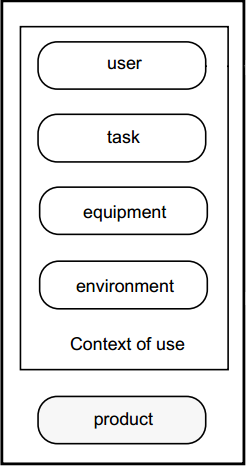
\includegraphics[scale=0.8]{contextOfUse.jpg}
\caption[Context of use]{Context of use, modified from \cite{contextofusefigure}}
\label{contextofuse}
\end{figure} 

\subsection{Simplicity}
\label{sec:simplicity}
Making good, intuitive, easy to understand systems is essential for a system to be successful, accepted and used. "Make it or break it" is a slogan that connects well with success and acceptance. A system can possess the best functionality there is, but if the users do not understand how to use it, the system will fail. An example of this is Apple's huge breakthrough when they launched their iPhone in 2007 \cite{iphone2007}. One might associate the invention of the touch phone with Apple's iPhone, but the truth is that touch phones was invented long before the iPhone. The first touch screen was published as early as in 1968, where it was used for air traffic control, and the first smart phone with touch screen technology was released early in the 1990s \cite{touchphone}. Apple was an eager participant in the development of touch screen devices. Already in 1983 Apple had a prototype of a touch screen phone \cite{applefirst1983}. Apple's success with their iPhone is based on focus on user's needs throughout the development process, which has resulted in good, intuitive and user-friendly design and interfaces. 

"KISS" and "Less is more" are other terms related to usability. "KISS" is an acronym that stands for "Keep it simple, stupid". This principle was formulated by the American aircraft designer Kelly Johnson in the middle of the 1900s, and it states that simple systems work better than complex ones. KISS is not related to stupidity, but rather to intelligent systems that due to their simplistic design may be perceived as stupid. The KISS principle has been adopted into software engineering, and subjects as design and usability. It states that simplicity should be the main focus in design, and that every element that leads to unnecessary complexity should be avoided \cite{kiss1} \cite{kiss2}. Ludwig Mies van der Rohe was a German architect that used the term "Less is more" to describe his extreme simplistic and minimalistic design style, and his use of that term became a guiding principle in modern design. "Less is more" has also been widely used as a slogan in association with usability. \cite{rohe}. Minimalistic design can be described as \emph{"design at its most basic, stripped of superfluous elements, colors, shapes and textures"}. With minimalistic design, the most important elements are brought into focus. In this way the user will not be distracted from, or miss out on, the content that is important \cite{lessismore}. Also big companies, like Microsoft, focus on simplicity in their design. Microsoft has launched an article called "The Importance of Simplicity" in their developer network. This is about how to design user-friendly systems while still keeping good functionality. Microsoft presents a topic called "Simple Can Be Powerful". This means that simplistic design not necessarily implies lack of functionality. Simplistic design will provide ease of use for first timers. The idea is to present a design that is intuitive, understandable and easy to learn, with a possibility for the experienced user to choose to add more functionality. A possible solution could be to include customisation so the users can set up their own workspace, and include more features if wanted \cite{msdnsimple}.            

\section{System Requirements}

To be able to make a system, designers must start with finding out what the system is going to be, what it should do and what functionality it should include. Finding out and documenting all this is called a requirement analysis. The requirements in this analysis should focus on the role and the purpose of the system, viewed from the environment. They should include what is essential to the system, and avoid details that are unnecessary. \emph{How} the system is going to realised, is not usual to include in these requirements. From a requirements analysis there is natural to produce what is called a requirement specification \cite{braude2000software}. Requirements specification is defined in \cite{systemutviklingDel1} as \emph{"A specification that sets forth the requirements for a system [...]. Typically included are: functional requirements, performance requirements, interface requirements, design requirements and development standards"}. The different requirements are often separated into two categorisations, functional and non-functional requirements. 

\subsection{Functional Requirements}
Functional requirements are about the system behaviour and the provided functionality \cite{systemutviklingDel1}, in addition it ways something about input/output devices, range of users etc. \cite{mmi}. \cite{systemutviklingDel1} mentions some examples of functional requirements:
\begin{itemize}
\item \emph{Requirements to ideal (functional) services and dialogues, possibly on several layers of abstraction.}
\item \emph{Requirements to ideal (conceptual) knowledge about the environment.}
\item \emph{Requirements to size: numbers of users, terminals etc.}
\end{itemize}     

Functional requirements will be used as a primary input to functional design. Functional design should say something about the complete functionality of the system that can be seen by the users, and is defined as \emph{"what the system shall do in a way that can be compared to the functional requirements. [...] it provides a basis for selecting the implementation. It is therefore idealised with respect to the concrete system and will hold for a range of technical solutions"}. Functional design is independent from technology and will not say anything about how the system is going to be implemented \cite{systemutviklingDel1}. 

\subsection{Non-Functional Requirements}
Non-functional requirements include performance requirements, interface requirements, reliability and availability requirements, error handling, and constraints. Performance requirements address speed, capacity and memory usage. Reliability and availability requirements specify reliability in quantitative terms, and the amount of time the system should be available to the users. Error handling is about how the system should respond to errors, and interface design says something about how the system will interact with the users. Constraints restrict how the system should be designed and implemented. This is done by describing accuracy, tool and language to be used, design constraints, which standards that should be used, and the hardware platform the system should be built upon \cite{braude2000software}. To summarise, non functional requirements are about ensuring quality of a system, and it says something about constraints on hardware, software, and the implementation of the system in general \cite{mmi}. Examples of non-functional requirements are mentioned in \cite{systemutviklingDel1} as:
\begin{itemize}
\item \emph{Requirements to (concrete) physical interfaces.}
\item \emph{Requirements to physical conditions like temperature, humidity, power, consumption etc.}
\item \emph{Requirements to processing capacity: response times, traffic load etc.}
\item \emph{Requirements to exception handling.} \\ \\ 
\end{itemize}   

Non-functional requirements form a basis for implementation design. While functional design is about what the system shall do, implementation design describes how the system should be realised. Implementation design connects the technical solution with the functional design, which makes the "manual" for how the final system will be implemented \cite{systemutviklingDel1}.  

An important part of developing a system is to decide and specify functional requirements and non-functional requirements. It is not always easy to distinguish between the different requirements, in terms of if they belong under the categorisation of functional or non-functional requirements. It is important to notice that categorisation of requirements is not the essential part. What is the main goal is to define and express the requirements as clear, simple and understandable as possible \cite{systemutviklingDel1}.    
  
\section{Design Guidelines}
\label{sec:designguide}
In order for a system to become successful it has to be easy to interact with, and it has to offer functionality that are attractive to the user. It is the work for an interactive system designer to combine system functionality with users needs. There have been developed several guidelines to help designers make successful, user-friendly systems. In this section we will present two of these guidelines, a theory about system design called "The Four Pillars of Design", and a list of eight principles with focus on interface design, called "The Eight Golden Rules". 

\subsection{The Four Pillars of Design}
\label{sec:fourpillarsofdesign}
The four pillars of design is not a theory that guarantees brilliant systems, but it could be helpful for an interactive system designer along the way in a development process. The four pillars of design consist of "user-interface requirements", "guidelines documents and processes", "user-interface software tools" and "expert reviews and usability testing" \cite{mmi}.    

\subsubsection{User-interface requirements (Ethnographic observations)}   
A major key to success when developing a system is connected to specifying the user requirements, and how well these requirements are defined and understood.  The way to specify requirements differs from system to system, but what the final result should always include is the same; Who should use the system, where should it be used and what should it be used for. 

\subsubsection{Guidelines documents and process (Theories and models)}
It is important for the interactive system designer to generate a document that obtains a set of guidelines which specifies how the design should be. This could be a design guidelines for the whole system, or it can be design guidelines for parts of the system, like functional design, implementation design, and interface design. Companies like e.g. Apple uses guidelines documents to specify design principles developers should follow. This is to create consistency in design across systems and products. Design may differ as different systems has different needs, but there are still some elements that should be considered in the guidelines document. It is important that the guidelines are flexible, so that they can adapt to changes in needs and experiences \cite{mmi}. Examples of what guidelines should describe are:

\begin{itemize}
\renewcommand{\labelitemi}{$\bullet$}
\item Words, icons, and graphics.
\item Screen-layout issues.
\item Input and output devices.
\item Action sequences.
\item Training.
\end{itemize}

\subsubsection{User-interface software tools (Algorithms and prototypes)}
In the early stages of development, it is difficult for users to picture what the final result will look like. One way to address this problem is to let the users get a realistic impression of the final result, by presenting different types of mock-ups and prototypes \cite{mmi}. What prototypes are, and how and when they should be used will be presented in Section \ref{sec:prototypes}. 

When deciding on which development environment to use, there are numbers of good products to choose from. Most of them are easy to use, and offers good features. The important part is for the developers to choose the development environment that is most suitable for the product they are going to make, due to performance, cost, and how easy it is to use and learn \cite{mmi}.
	
\subsubsection{Expert reviews and usability testing (Controlled experiments)}
To be able to launch a successful system, it is important with testing along the way in the development process. System testing could involve both experts and the intended users \cite{mmi}. 

\subsection{The Eight Golden Rules}
\label{subsec:golden}
The "Eight Golden Rules", presented in \cite{mmi}, are a set of guidelines that has been developed over three decades with research and experiences. There does not exist a solution for how to make good and user-friendly interface design, but these "Eight Golden Rules" can serve as a starting point and a helpful design guide if they are used correctly. When using the "Eight Golden Rules", it is important that designers refines and implements the principles into the environment they are working in. 

We will now present the "Eight Golden Rules".

\begin{itemize} 
\item \emph{Strive for consistency:} Consistency in interfaces requires identical terminology for actions and layout. This is important for users not to wonder whether words, icons or situations means the same. 
\item \emph{Cater to universal usability:} Designers have to see the need for making a design that fits the diversity of users. There could be differences in age and technology experience, that requires transformation of content. Beginners would need guiding and explanations, while experts should have features for short cuts. This could improve quality of the system experience. 
\item \emph{Offer informative feedback:} The users should always receive feedback on their actions. Appropriate system feedback should be chosen in accordance to the importance of the actions performed. Process bars, sound as a response for clicking a button, or visual presentation for showing object in actions, is possible ways to give users feedback on actions.  
\item \emph{Design dialogues to yield closure:} It is important to create distinct work steps in dialogues. This means organising similar actions into separate groups with a clear start, middle, and an ending. To provide users with a feeling of accomplishment, feedback should be provided when a particular sequence is finished.     
\item \emph{Prevent errors:} The best solution to this problem would be not to experience any errors at all. Designers should prevent users from doing serious errors by e.g. not allowing inappropriate digits in a field or "hiding" buttons that could cause errors. However, when errors do occur users should be provided with informative instructions for how to recover from the problem.   
\item \emph{Permit easy reversal of actions:} Users should always be provided with the possibility to regret a performed action. This will make the system easy and comforting to use, as users know that every action can be undone. 
\item \emph{Support internal locus of control:} User should feel that they are controlling the interface, and not the other way around. This might be especially important for experienced users. Surprising changes in design and actions, in addition to boring, time-consuming situations, will not be well received. 
\item \emph{Reduce short-term memory load:} Designers should reduce the need for memorising information and how actions should be performed. The focus should be on designing an interface with visible information and intuitive actions.
\end{itemize}

These presented guidelines are far from being the only guides for how to design a user interface. There have been done a huge amount of research in the area of usability, where Jacob Nielsen is one of the participants \cite{nielsen2005ten}. Nielsen is a Ph.D from Denmark, and an expert in human-computer interaction. He has established a movement for how to easy improve user interfaces, invented several methods for how to achieve good usability, and he has also published a great amount of articles and books with usability as main subject \cite{JNielsen}. As a part of his work Nielsen has created a list of ten usability heuristics, which can be used as general principles when designing a user interface\cite{nielsen2005ten}. We will discuss this in Section \ref{sec:heur}. Now, we will present difficulties and possible solutions related to developing interfaces for elderly users.

\subsection{Designing User-Friendly Interfaces for Elderly Users}
\label{sec:designelderly}
The world's population is ageing, in addition to people living longer. This together with baby boomers has led to a great share of older people in the world. In 2007, 20 percent of the population in the developed world was over the age of 60 \cite{dickinson2007methods}, and it is expected that 25 percent of the population in Europe will be over the age of 60 by 2020 \cite{ijsselsteijn2007digital}. 

Use of technology for different purposes has become an important part of peoples' everyday life. However, many older people do not use technology as computers, mobile phones, tablets, etc., because it is unfamiliar to them. In fact, some of them says they are afraid of using this new technology because they feel they would not master it \cite{mmi}. Even though this is the case, many elderly are interested in the functionality the technology provides, and they are eager to try and to learn more about it. By including elderly in the use of technology, both elderly and the society will experience benefits. Elderly will be able to write emails to stay in touch with family, they could pay bills, share photos, entertain and educate themselves through different games, etc. It is also shown that elderly are attracted by computer and video games \cite{mmi} \cite{ijsselsteijn2007digital}, because it stimulates social interaction. In addition, video games provide them with challenges that could give them a feeling of mastery and higher self-confidence \cite{mmi}. 

Most of the research done on human-computer interaction are performed on young people \cite{dickinson2007methods}, but with the wave of elderly ahead of us interface designers has to put a greater focus on older people and their needs when developing new systems. Especially, this means taking disabilities due to ageing into consideration. As mentioned in Chapter \ref{chap:exforseniors} will ageing often lead to both physical and psychological negative changes, like decline in cognitive skills, visual and auditory acuity, and in balance and physical strength. Elderly will also experience memory loss, and difficulties moving around due to decreased flexibility. When working on interface design, visual decline may be the most important aspect to focus on. Visual decline implies less contrast sensitivity, decrease in peripheral vision, and more dark adoption. 

There exist various examples of guidelines for how to design good and user-friendly interfaces for elderly, or people in general, that are partially sighted or visually impaired. Some of the main guidelines are simple design, large font size, and sharp contrast between background color and font color. The users might have different levels of visual decline, so it is preferable to allow users to change settings themselves \cite{blindeforbundetTekst} \cite{actionforblindpeopleTekst} \cite{w3cTekst}. These design guidelines are provided by various organisations, as e.g. "Blindeforbundet", a Norwegian federation for everyone with poor vision \cite{blindeforbundet}, "Action for blind people", a charity in the UK which provides support to people that are blind or partially sighted \cite{actionforblindpeople}, and "World Wide Web Consortium (W3C)", a community working together to create web standards \cite{w3c}. These web standards are meant to be used as guidelines for making usable interfaces for the general user, regardless of age or disabilities \cite{w3cTekst}. These three organisations are just a few out of several others with focus on making technology accessible for elderly and people with visual disabilities. 

We will now present a summary of guidelines to consider when designing an interface for elderly, mostly gathered from the three organisations mentioned above.

\begin{figure} [ht!]
\centering
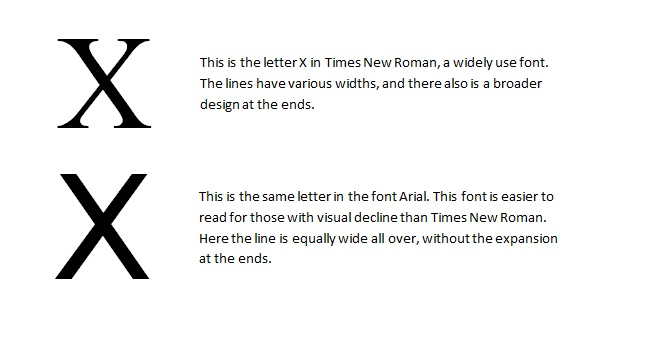
\includegraphics[scale=0.9]{fontExample.jpg}
\caption[Fonts]{Font with and without serifs [modified from \cite{blindeforbundetTekst}]}
\label{fig:fonts}
\end{figure}

\textbf{Make the text easy to read}
\begin{itemize} 
\item Use a relatively large font size, minimum 12 pt \cite{blindeforbundetTekst} \cite{evengrounds}. A font size of 14-16 pt is preferable for those who are visually impaired. For large prints use 16-22 pt \cite{actionforblindpeopleTekst}. Use of font size larger than 20 pt will not increase readability in a text.     
\item Use a clear print. This mean that a sans serif font should be used, see Figure \ref{fig:fonts}. Arial, Helvetica and Futura are fonts that are easy to read \cite{actionforblindpeopleTekst}.
\item Avoid fonts with special styles \cite{blindeforbundetTekst} \cite{actionforblindpeopleTekst}.
\item For titles, use upper-case letters in beginning of words \cite{actionforblindpeopleTekst}. Do not use capital letters in large amounts. They give little variation, which makes the text difficult to read \cite{blindeforbundetTekst}. 
\item Do not use italics, underlining and bold typing in a larger coherent text, that will disturb the reading \cite{blindeforbundetTekst} \cite{actionforblindpeopleTekst}.  
\item If possible, allow the users to change font and text settings themselves \cite{blindeforbundetTekst} \cite{w3cTekst}. 
\item Use a language with ordinary, well-known words. This makes the text more easy to understand \cite{w3cTekst}. \\ 
\end{itemize}

\textbf{Use simple design}
\begin{itemize} 
\item Use simple design, as this makes it easy for important elements to stand out \cite{actionforblindpeopleTekst}.
\item Be consistent in design and layout throughout the system \cite{actionforblindpeopleTekst}.
\item Always use left-aligned text. Centered text appears unclear \cite{actionforblindpeopleTekst}.  
\item Keep spacing between words permanent. Do not stretch the text to get an even right margin, as this will change the spacing randomly. An uneven right margin is good for readability, as it help leading the eyes to the next line \cite{blindeforbundetTekst} \cite{actionforblindpeopleTekst}.
\item Do not use to much or to little spacing between lines \cite{blindeforbundetTekst} \cite{actionforblindpeopleTekst}. 
\item Avoid big blocks of text. The text will be easier to read and understand if it is divided into smaller sections \cite{blindeforbundetTekst} \cite{actionforblindpeopleTekst} \cite{evengrounds}. \\  
\end{itemize}

\textbf{Use of colors and contrasts}
\begin{itemize} 
\item It is important with sharp and clear contrast between background color and font color to ensure good readability \cite{blindeforbundetTekst} \cite{actionforblindpeopleTekst}. The actual choice of colors is not that essential.   
\item In general, the most preferred combination of background color and font color is black text on either white or yellow background \cite{actionforblindpeopleTekst}. Black on white or yellow creates very good contrast \cite{blindeforbundetTekst}. 
\item People are different. Some might prefer the opposite, like light font colors on dark background \cite{blindeforbundetTekst}. This again emphasises that it should be possible to customise settings. When using light font colors on dark background, the font should be both bigger and bolder to make the text more readable \cite{actionforblindpeopleTekst}.
\item Avoid pale colors on colored background \cite{blindeforbundetTekst}.  
\item Choose a one-colored background. Try not to write text on pictures. The picture will take the attention away from the text, and make the text harder to read. If necessary, put the text where there is light areas in the picture  \cite{blindeforbundetTekst}.  
\item Reading speed and distant reading is also highly connected to colors and contrast  \cite{blindeforbundetTekst}. Black text on white background provides the highest reading speed in a text. For more combinations, see Figure \ref{fig:colors}.
\end{itemize}

\begin{figure} [ht!]
\centering
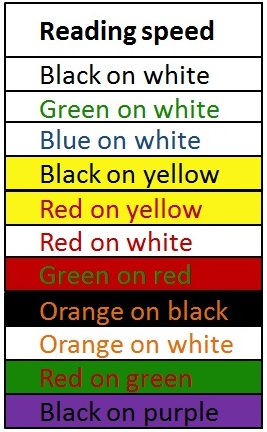
\includegraphics[scale=0.8]{readingcolors.jpg}
\caption[Colors and contrasts]{Relationship between reading speed and distant reading, and colors and contrasts. The best combinations are those shown on top [modified from \cite{blindeforbundetTekst}]}
\label{fig:colors}
\end{figure}

\textbf{Provide necessary information}
\begin{itemize}
\item Provide alternatives for how to present information. For those who are visually impaired, an audio presentation might be preferable \cite{blindeforbundetTekst} \cite{w3cTekst}. 
\item Text is a better way to present information than use of images and icons \cite{w3cTekst}.
\item Give the users time to read the given information. Let them tell the system when they are finished reading \cite{w3cTekst}.  
\item Help users to easily navigate to the the content of interest \cite{w3cTekst}.
\item Assist users on how to avoid and correct mistakes. Describe the error for the user, and provide a suggestion for how they can undo the action that caused the error \cite{w3cTekst}.      
\end{itemize}

\section{Heuristics}
\label{sec:heur}
Heuristics are designed guidelines made to assess how good software design is, and it has become a widely used method for usability evaluation in software development. It is important to develop software interfaces that are easy to understand, learn and conduct. With the use of heuristic, this can easily be evaluated. Heuristic evaluation method allows for insight into users' point of view, even before there is an actual system, and is actually best suited in an early phase, before spending a lot of money on expensive prototypes.  When prototypes are made, the user needs to be involved to discover problems if they appear. This is also a very important part of the development, because it is critical to understand the interaction between the player and the game \cite{desurvire}. As mentioned in \ref{subsec:golden}, Jacob Nielsen developed a set of heuristics which can be used as guidelines when developing user interfaces. These can be found in \cite{nielsen2005ten}. However, these heuristics are made for software development in general. We sought to find heuristics that were more applicable for game development. 

We found that a lot of research have been done and that there has been suggested different sets of heuristics in addition to the ten heuristics suggested by Nielsen \cite{nielsen2005ten}. Some worth mentioning are Desurvire et al. \cite{desurvire}, Malone \cite{malone}, Shelley \cite{shelley}, and Federoff \cite{federoff}. Many of these overlap, and in some way, they all tell the same.  Desurvire et al. presents a thorough set of heuristics that covers four game heuristic categories:  \emph{Game play}, which is the challenges that needs to be overcome to win the game, \emph{Game Story}, which intuitively is the story of the game and its characters, \emph{Game Mechanics}, which covers the interaction between objects and the game environment, and  \emph{Game Usability}, which is the elements used to be able to interact with the game, like for example a controller. They present a set of heuristics that is based on the already existing literature. The heuristics have also been reviewed by different playability experts and game designers. The model presented by Desurvire et al. proved to be very useful in an early development phase \cite{desurvire}.

Melissa Federoff evaluates in her thesis different sets of heuristics from the literature. With these in mind, she did a case study where she observed and interviewed different members of a game development team. Based on the findings she did she removed some heuristics, added some heuristics, and  suggested a new set of heuristics. The list of heuristics that she created in her study can serve as a starting point for the development of a standard list that the game community can use  \cite{federoff}. 

Even though Federoff's study was aimed towards game development, Sweetser and Wyeth discovered that many of the heuristics proposed in the literature, did not evaluate the enjoyment in games. They argue that the many valid sets of heuristics presented in the literature should be integrated in a model where also player enjoyment can be assessed. How much someone enjoys something can be described by the concept of flow. The concept of flow was first proposed by  Mihaly Csikszentmihalyi, when he many years ago started  to study how people could be so immersed and engaged in something they did not get money for. He wanted to find out why they did these things. He found that the reason was the enjoyment they felt when doing it. He called this state "flow" because "many of the respondents described the feeling when things were going well as an almost automatic, effortless, yet highly focused state of consciousness" \cite{flow}.  Sweetser and Wyeth integrated the already existing heuristics into the model of "flow", and called this new model "GameFlow".  They argued that the nature of flow fits well as a way to structure the different heuristics found in the literature, into a model of player enjoyment. The "GameFlow" model has eight core elements which are related to Csikszentmihalyi's defined elements. The core elements are: \emph{concentration, challenge, skills, control, clear goals, feedback, immersion} and \emph{social interaction}, see Figure \ref{fig:gameflow1} and \ref{fig:gameflow2} \cite{sweetser}. 

\begin{figure} [ht!]
\centering
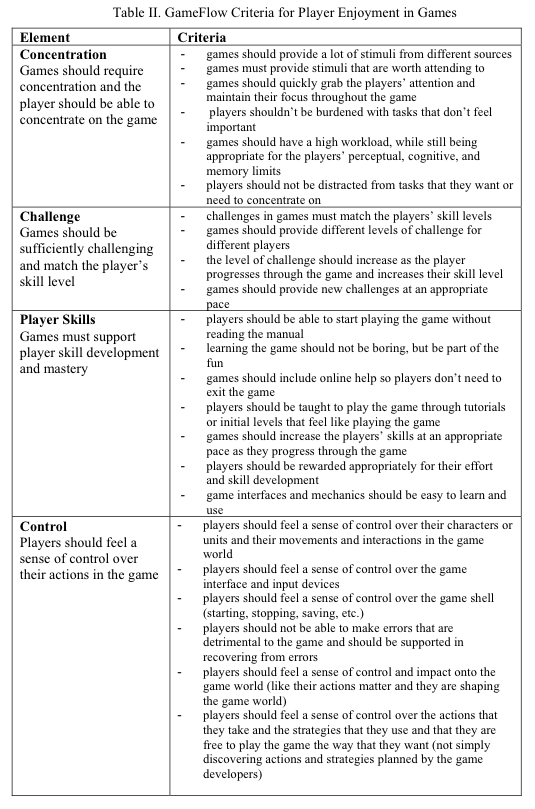
\includegraphics[scale=0.9]{gameflow1}
\caption[GameFlow criteria for player enjoyment in games, part 1]{GameFlow criteria for player enjoyment in games, part 1 \cite{sweetser}}
\label{fig:gameflow1}
\end{figure}  

\begin{figure} [ht!]
\centering
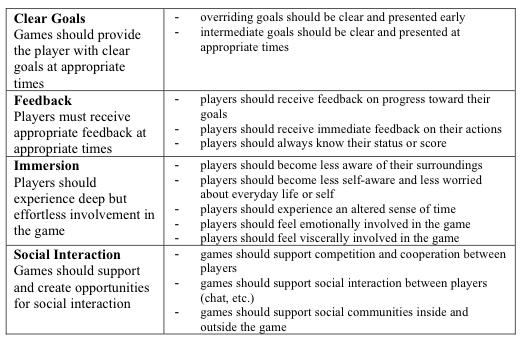
\includegraphics[scale=0.7]{gameflow2}
\caption[GameFlow criteria for player enjoyment in games, part 2]{GameFlow criteria for player enjoyment in games, part 2 \cite{sweetser}}
\label{fig:gameflow2}
\end{figure}  

We will now discuss the eight core elements briefly. We will not discuss every criteria, as they are all presented in Figure \ref{fig:gameflow1} and \ref{fig:gameflow2}, but we will emphasis some of the elements we find important. 

For the game to be fun, the player needs to be able to concentrate on the tasks. The players attention and concentration should be maintained throughout the whole game time. The tasks have to give meaning to the player and unnecessary tasks should be avoided. Challenge is important because this is what makes a game fun. It is not fun to play something that is too easy, and it is definitely not fun to play something that the player is not able to do. Therefore, it is important that the challenge match the players' skill level. This can be done by providing the possibility to vary difficulty level and pace. Commonly it is very satisfactory to overcome hard challenges. The game should start out at an easy level, and then increase in difficulty as the player plays along. The game should also have different possibilities for the player to develop new skills. The way in which the player learn how to play the game is also important and should be provided in an interesting way. Learning the game should also be a part of the fun. A common method, is to learn as the player plays. It is important to reward the players appropriately as they accomplish challenges.  Games should be self-explanatory, and not require any long manuals to be read before playing. The player needs to feel that they have control over the actions they are performing in the game. The player should also be in control when to start, stop and save the game. Different actions that can be done, as well as the choices in the menu, should be intuitive and easy to understand. The players different actions, should have an impact on the game play. It is important to give the player freedom, including giving the player options, multiple ways to go, and multiple ways to win a game. The game should have clear goals, and the player should be aware of them at appropriate times. The game should have one main goal, but also multiple goals at different levels. Feedback should be provided at appropriate times. This feedback should say something about their progress, scores, and encouraging messages. The game should capture the player so that the player is really involved in the game. Audio and the game story are important to gain immersion. An other important aspect to consider with video games is social interaction. In \cite{sweetser} they discuss how social interaction is not a flow element, and how it can interrupt immersion. This is because real people can get the players "back in the real world". However, it is seen as a very important aspect, as many people play games for social interaction \cite{sweetser}.

The model was tested on two strategy games "World of Warcraft" and "Lords of EverQuest", and it was found that not all criterias were applicable to strategy games, suggesting that different criterias suite different genres. Some of the criterias would also need to involve the player to evaluate, for example when deciding if a game suits different skill levels. However, the paper suggest that the "GameFlow" model can be used as guidelines for an expert review, or as suggested in Desurvire, guidelines in an early phase \cite{sweetser} \cite{desurvire}. 

In this thesis we will develop a game concept in an early phase. As learned from this chapter there is very important to involve the user to make a user-friendly technology system. The set of heuristics suggested by Sweetser and Wyeth, and presented in Figure \ref{fig:gameflow1} and \ref{fig:gameflow2}, will be used in our work, as we found these to be valuable guidelines, and because we believe it is especially important to evaluate the enjoyment of the game, in this kind of persuasive game (si noe mer om persuasive games ett sted).  We will now move on to the next chapter, where we will discuss the methods used to involve the user in the development process.

(With the importance of user friendly technology systems, was well as user involvement, in mind, we will move on to the next chapter, where we will describe the methodology used in this thesis. )